\label{chap_kmc400}



The Kangaroo foundation has contributed significantly to the development of this project. The experts that work with the foundation have provided us information on their research methodologies. They also provided us two very interesting data-sets and were willing to test all our prototypes. In return we helped them analyze and make sense of these complex data-sets. This collaboration enriched the project and allowed the experts in the foundation to extract information from the data efficiently. This chapter will illustrate the benefits of this collaboration and show how the Braviz platform can provide value in a real study. Notice that the full methodology and results from this study can be found elsewhere \autocite{charpak_final_2015}; in this chapter only some aspects are illustrated in order to provide the context in which the tools were used.

\section{Kangaroo Mother Care}

%cual es el problema?
Low birth weight (LBW) is a mayor cause of child mortality \autocite{wardlaw_low_2005}. On those who survive it can produce long term sequels and impairments \autocite{nosarti_neurodevelopmental_2010}. 

Kangaroo mother care was developed by Edgar Rey in 1978 \autocite{rey_rational_1983} as an alternative to the conventional method of care for infants born with low weight \autocite{conde-agudelo_kangaroo_2003}. It was initially conceived to deal with the lack of incubators and high rate of infections. In KMC the mother is used as a source of heat to keep the child warm. In this way it is also possible to let mother and child leave the hospital earlier, and therefore keep the baby away from possible infections. There are three main components in the treatment.

The first one is kangaroo position, where the child is placed on the mother's or father's chest skin to skin in an upright vertical position. This has the effect  of keeping the baby warm, and provides positive stimulation to the babies brain through all senses. In kangaroo position the baby hears the mother's voice and her heart beat, senses her smell, feels her skin ans sees her face and her environment \autocite{tessier_kangaroo_2003}. Additionally the mother receives the stimulation she needs to increase milk production \autocite{charpak_kangaroo_2005}. This positions is maintained until the baby doesn't tolerate it any more, which indicates that appropriate temperature regulation has been achieved. 

The second component is nutrition by breast milk every two hours. The goal is to obtain a weight gain rate similar to what it would be in uterus. If the baby's growth is shown to be adequate the feeding schedule can be relaxed. In case the target weight gain can't be accomplished with breat milk alone, a formula supplement may be added. However it is important to administer this supplement via dropper or spoon so that it doesn't interfere with breastfeeding.

The final component is an early discharge from the hospital, with proper followup. This has the benefit of keeping the child away from infections, as well as providing an environment where strong bonds between the child and his family are more likely to form \autocite{charpak_kangaroo_2005}. 

\begin{figure}
    \centering
    \begin{subfigure}{0.45\textwidth}
        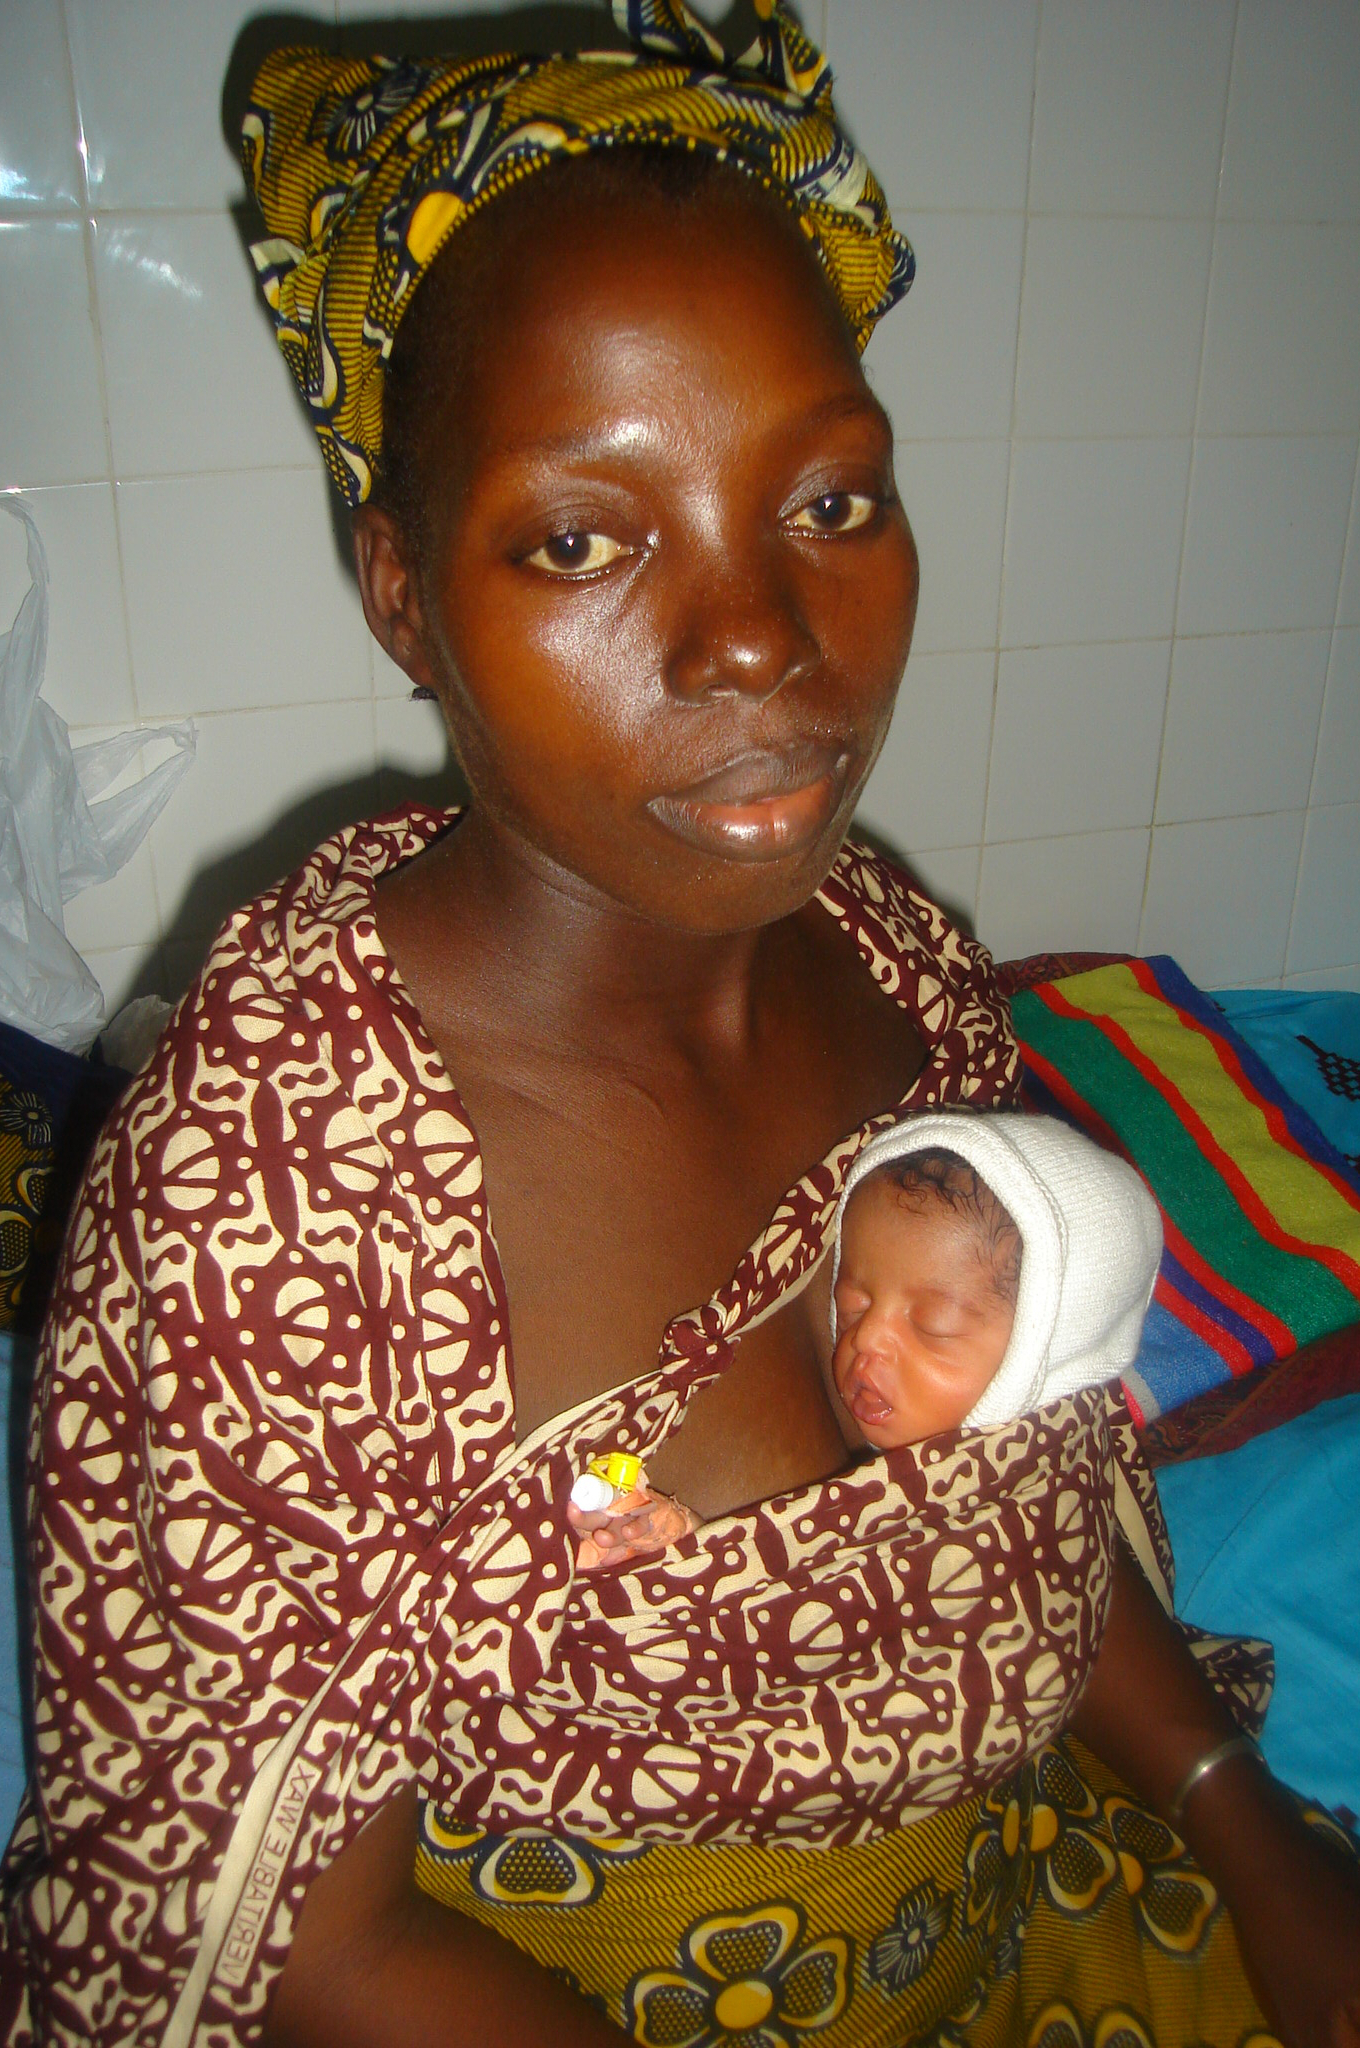
\includegraphics[width=\textwidth]{kmc400/221_trimmed}
    \end{subfigure} ~
    \begin{subfigure}{0.45\textwidth}
        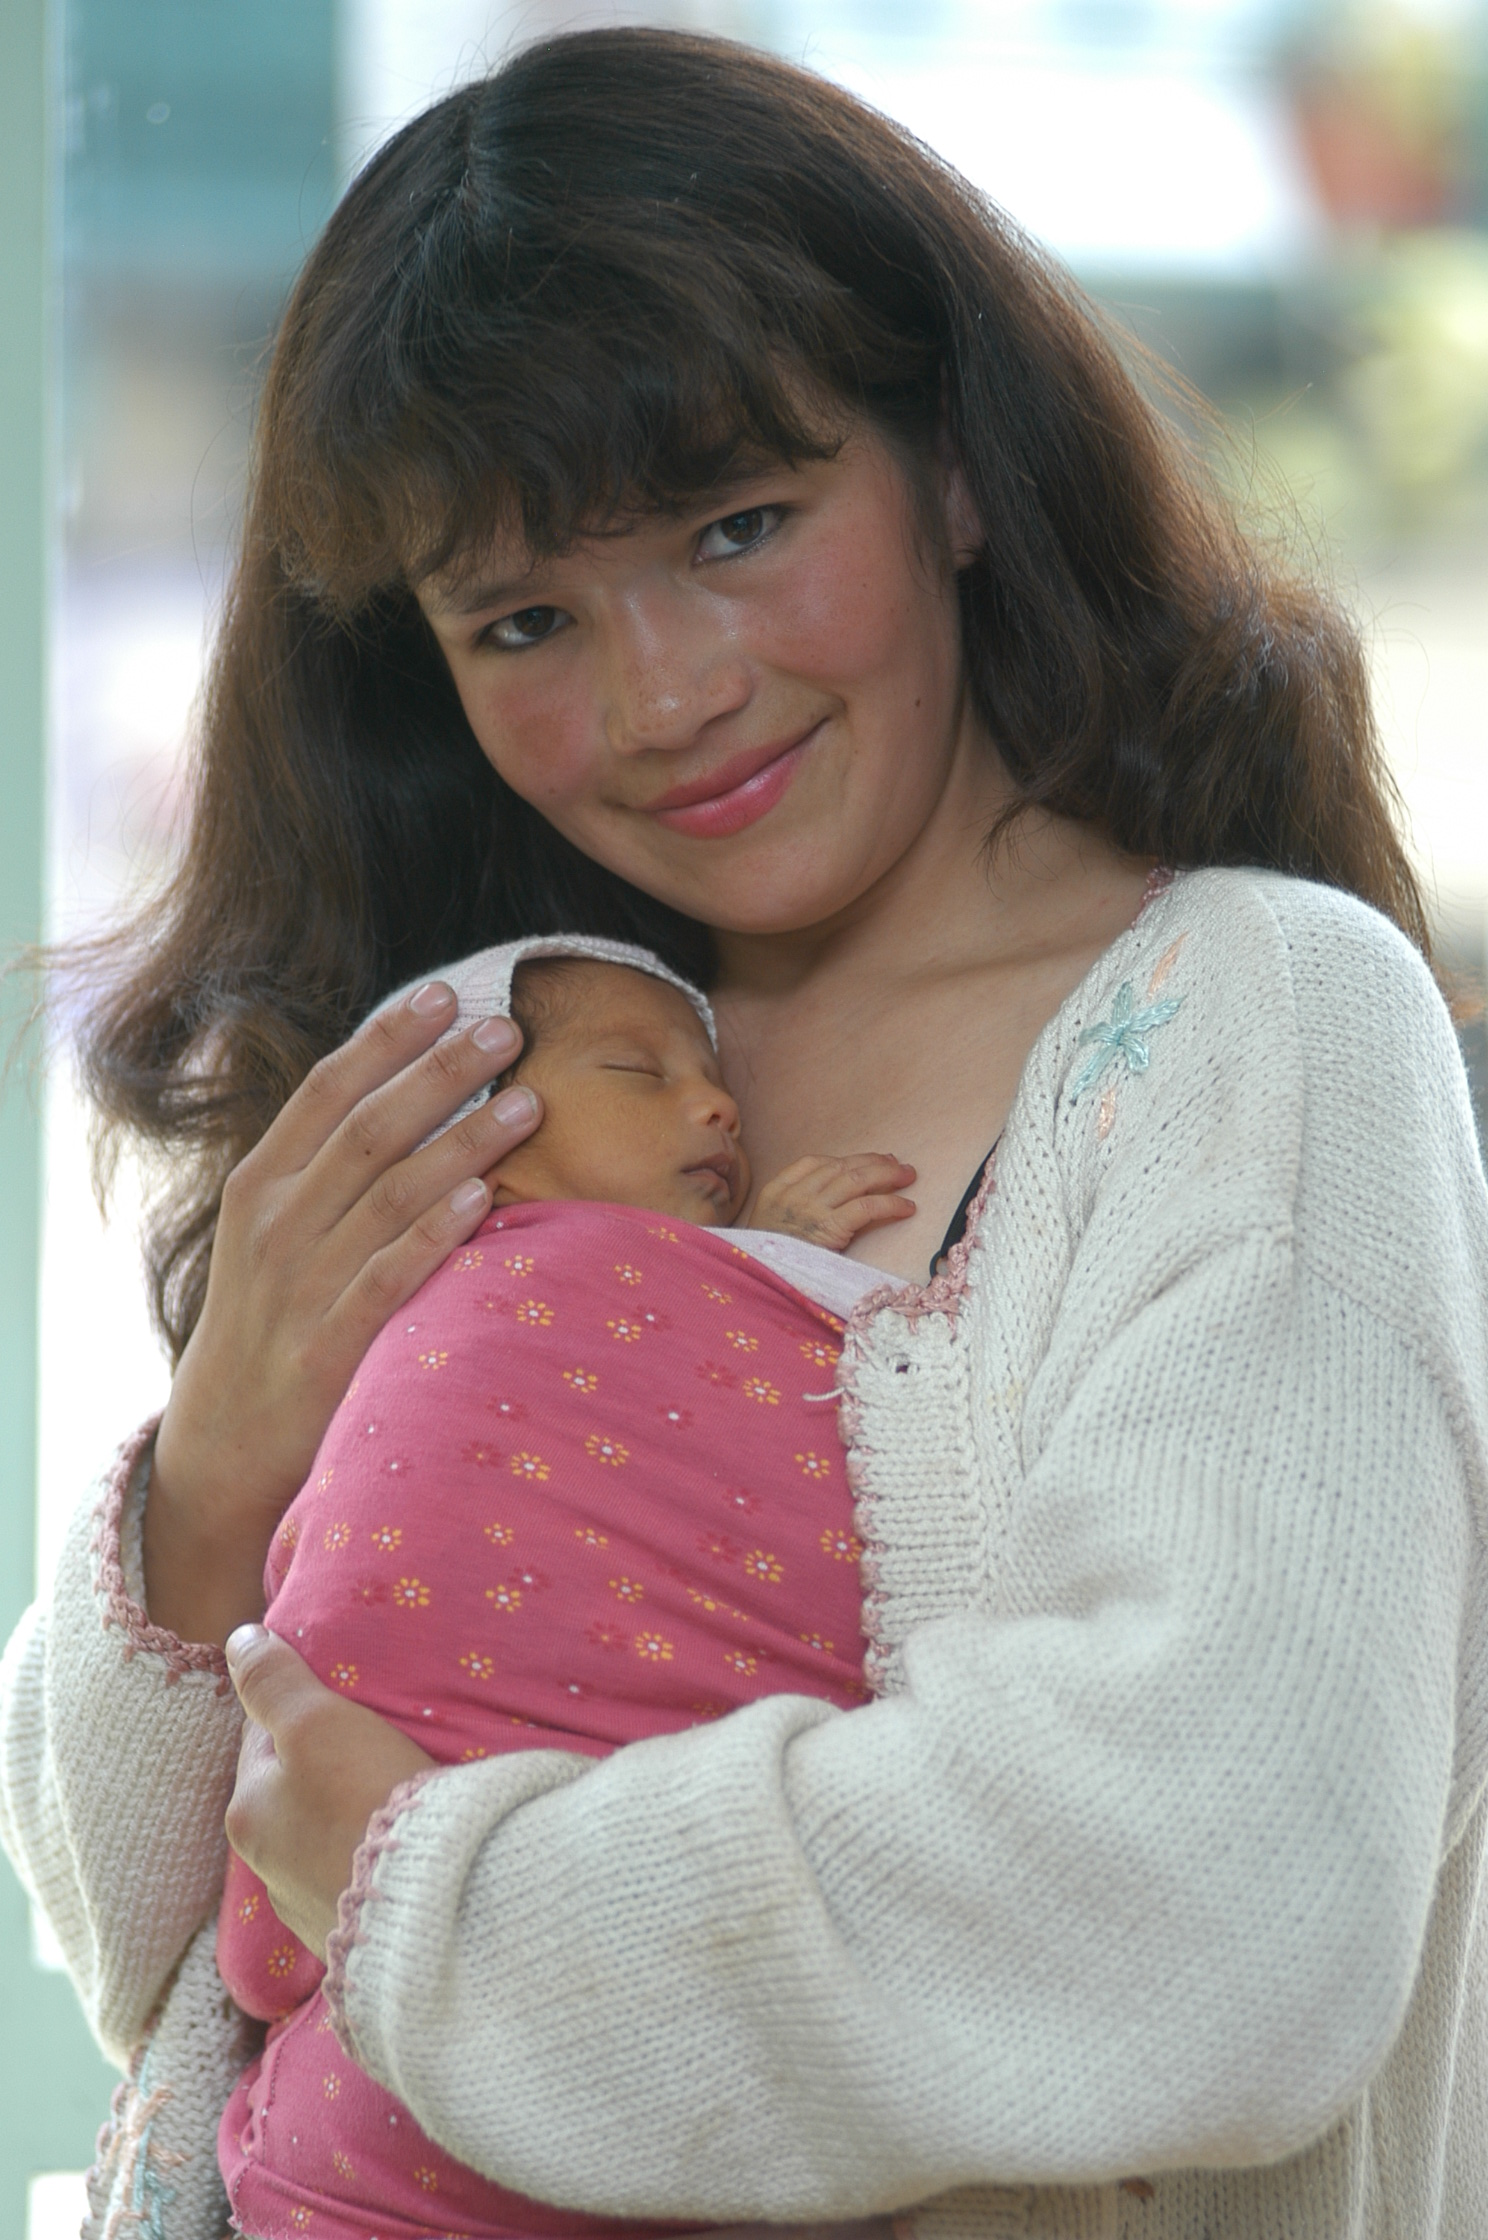
\includegraphics[width=\textwidth]{kmc400/0503canguro4d}
    \end{subfigure}
		\par \bigskip
		\begin{subfigure}{0.45\textwidth}
        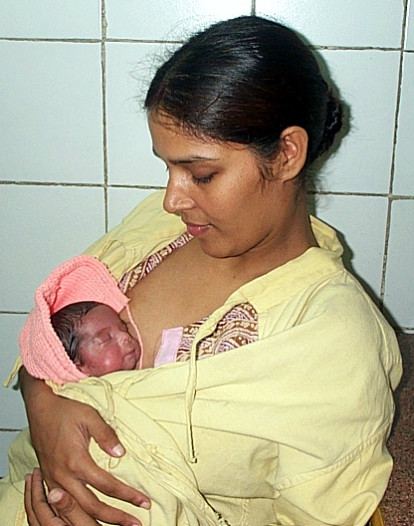
\includegraphics[width=\textwidth]{kmc400/Inde}
    \end{subfigure} ~
		    \begin{subfigure}{0.45\textwidth}
        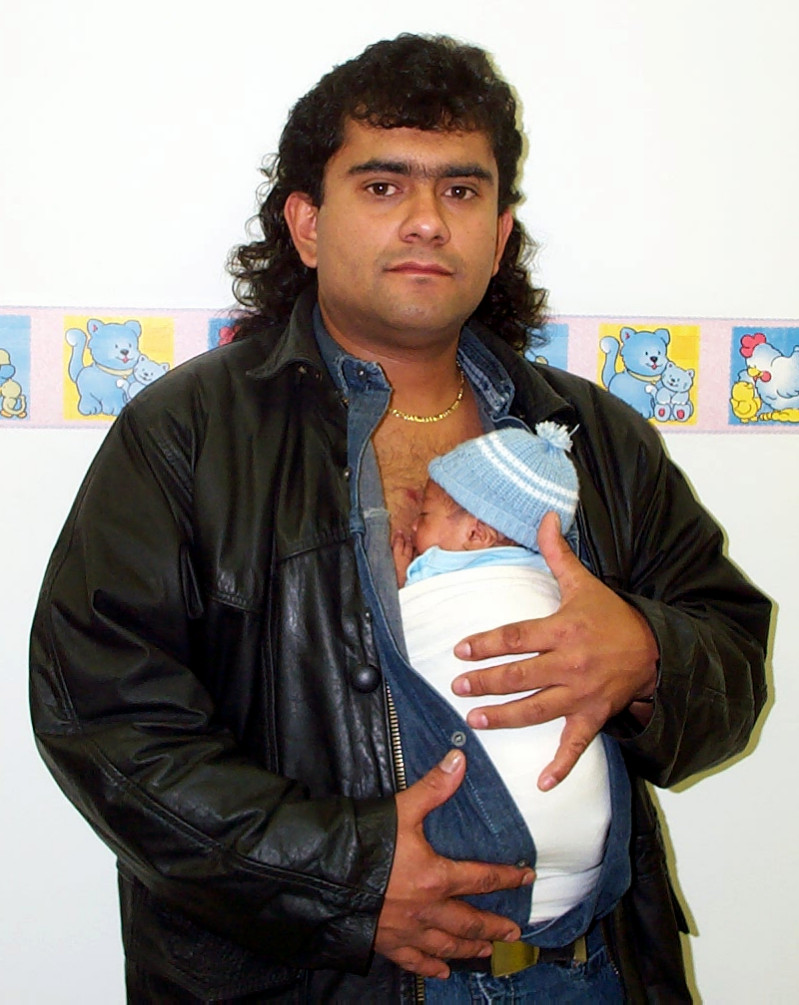
\includegraphics[width=\textwidth]{kmc400/papa2}
    \end{subfigure}
    \caption{Examples of the Kangaroo position, copyright belongs to the Kangaroo Foundation, used with permission}\label{fig_kmc_position}
\end{figure}

KMC has gone a long way since its invention \autocite{charpak_kmc_2011} and several refinements has been developed. For instance, the kangaroo position is now started as soon as the baby is born whenever its possible. Several research has been conducted on the method which has provided a better understanding of its benefits \autocite{the_cochrane_collaboration_kangaroo_2014}.
Kangaroo mother care has been adopted by the world health organization as a major strategy to decrease neonatal mortality in low birth weight infants. The kangaroo foundation is present in 30 countries with 60 teams. 


%- What is KMC
%http://www.fundacioncanguro.co/en/quienes-somos.html
%(preguntar a Rejean y Nathalie)

\section{Randomized Control Trial}
%- The first randomized trial

Between 1993 and 1996 a randomized controlled trial comparing short and middle term outcomes of KMC in comparison to traditional treatment was conducted. The sample consisted of 746 infants born with low weight (less than 2000g.) at \emph{Clinica San Pedro Claver} in Bogotá. Eligible infants were randomly assigned to either KMC or traditional incubator treatment. KMC group remained on kangaroo position 24 hours a day and nurtured by breast feeding and an optional supplement (preterm infant formula) delivered by spoon or dropper, in order to guarantee a weight gain of 15 grams per kilogram per day until the reach of term. Children in the traditional group were kept in an incubator until they were able to control their temperature and were gaining weight at an acceptable rate, and discharged according to standard hospital practice. Both groups were followed until one year of corrected age. 

%-- What were the main findings
During this year there were fewer deaths in the KMC group as well as fewer visits to the hospital caused by infections. In addition, competency tests showed that mothers from the KMC group felt more competent with their babies. Griffiths and INFANIB tests showed higher cognitive development in the KMC group. This effect was more prominent on those born before 32 weeks of gestational age and those who went through ICU. There was also a high impact of KMC on the development of personal relations and on planning functions related to brain development \autocite{tessier_kangaroo_2003}. Details of this study and its findings can be found in \autocite{charpak_current_1996,charpak_kangaroo_1997,charpak_randomized_2001,charpak_kangaroo_2005}.


%\autocite{charpak_kangaroo_1997}
%\autocite{charpak_kangaroo_2005}
%\autocite{charpak_randomized_2001}
%\autocite{charpak_current_1996}

\section{Pilot Study}

%The pilot study
% - Data
% - TMS findings
% - IMAGINE

In 2009, thirty-nine children who were part of the original study were relocated. The sample was composed of children born at or before 33 weeks of gestational age, 21 belonged to the KMC group and 18 from the traditional group. In addition, 9 kids born at term at the same hospital were recruited. 
The first step was doing full sight and hearing exams and, in case of need, prescribing and manufacturing glasses or hearing aides. One month was given in order to let the children adapt to glasses. Afterwards they went through several neuropsychological tests including Wisc, VMI, and CBCL. They also went to a TMS experiment and magnetic resonance imaging (MRI), where structural T1 and T2 weighted images were captured together with DWI and six functional paradigms. This data was acquired at \emph{Fundación Santa Fé de Bogotá} using a GE Sigma HD scanner of 1.5 Tesla. 

%¿Que se hizo con estos datos?

%¿What tests?

%¿Resultados imágenes?

%¿Qué se hizo con las imágenes?

%¿Alguna otra publicacion?


Functional images were processed with FSL and DWI images were processed using MEDINRIA. Additionally several anatomical regions were segmented and measured manually. he KAB software platform described in section \ref{sec_kab} was developed to perform additional analysis on this data. This tool was appreciated by researchers as it provided a link between quantitative data and the spatial data from which it is derived. It also created an environment in which it was possible to think visually of the relationships between TMS, white matter structure and functional MRI. This dataset was also used for testing and validating the first versions of Braviz (see section \ref{sec_iterations}).

The TMS study in this pilot showed an important difference in kids that belonged to the incubator group compared to those in KMC and term \autocite{schneider_cerebral_2012} in inter-hemispheric inhibition. The latency of this inhibition also showed some interesting effects in the interaction between gender, hemisphere and group. This results indicate that KMC encourages brain plasticity and therefore reduce the effects of a preterm birth. 

% Parallel with braviz development in the previous section

\section{Saving Brains Project}

%Teams : images, psycho, economists, medical, eyes, social workers, 

% - Objectives
% - Data Collection
% -- Process
% --- how?
% --- when?
% -- Participants


%The saving brains project

Between 2013 and 2014, financed by Canada Grand Challenges, the kangaroo foundation started a project that involved relocating and recruiting 50\% of the subjects from the RCT that survived after the first year (between 340 and 430 subjects). Measures were planned in order to avoid selection bias in this sub-sample. Specifically, comparing the distributions of relevant demo-graphical and clinical variables between the retrieved and not retrieved groups, as well as comparing them between the two groups (KMC and control) in the retrieved population. In case a selection bias was detected sensibility analyzes would be conducted on any results in order to mitigate the effects. 

Given budget restrictions it was not possible to perform magnetic resonance scans on the whole sample. However the initial RCT was stratified by birth weight, which allowed to make unbiased comparisons on each stratum. Therefore, it was decided to do imaging only on those participants which were born with less that 1800 g. 

By this time participants were between 18 and 20 years old. The study aimed at identifying if the KMC intervention had a long term effect protecting the brain against cognitive, social, and academic difficulties. Specifically, by analyzing data about brain maturation and structure, mental functions and behavioral patterns exhibited in family, school and work. 

Because there were no reference values for young adults available for some of the neuro-psychological and functional imaging paradigms that were to be acquired a complementary sample of fifty subjects born at term on the same clinic where the RCT was performed was also retrieved. This sample was part of an observational study that occurred one year after the main RCT. This sample was meant only to provide reference values, not for direct comparisons with the other groups.

Relocating the subjects started by using the contact information from the original RCT; followed by searches in government databases and social networks, public media advertising and visits to the last known residency where information was sought from current inhabitants and neighbors. This labor was conducted by the social workers in the foundation, at the end managed to relocate 491 subjects, from which 441 could and were willing to participate in the new study. 


%phases of the study
 
As in the pilot study, the first stop for each participant is a vision and hearing examination, following by the prescription and acquisition of glasses or hearing aides if they were needed. After one month or habituation, data would be collected on tree different days.

The first day comprised a full medical evaluation where the medical history was collected and physical and neurological exams were performed by a pediatrician. During the exam quality of life (Kidscreen-52) and Life habits surveys were administered. Afterwards a battery of neuro-psychological tests were administered by a psychologist. Details of these tests will be given in a following section. 

On a second visit the TMS experiment was conducted, and magnetic resonance images were acquired for subjects born with less 1800 g. of weight. Details of TMS and MRI scan will be presented later.

Finally, the social worker and an economist visited the residency, place of work and school of the participant. In this visit an evaluation of the dwelling place was conducted, and questionnaires were applied to parents and best friend. If the subject was at school a class play test was performed in the classroom. Finally the economist retrieved information about the education and work history of the participant, and collected the necessary information and authorization to retrieve the results of the national high school test (saber-11).

In addition, data captured during the first year follow up were retrieved from the database. These include

\begin{itemize}
\item Social characteristics of parents
\item Pregnancy characteristics 
\item Type of birth
\item Weight, size and cranial perimeter at birth and during follow up
\item Hospitalization at birth and during follow up
\item Questionnaire of mother competence
\end{itemize}

Data was captured in paper and online using standarized forms. These data was then entered into an Microsoft Access Database specifically implemented for the project. Data cleaning and quality control processes were performed regularly during data acquisition. These included double data entry for selected variables and manual comparison of database values and raw data. Periodic exploratory analyzes were also conducted regularly while data was being acquired. These allowed to quickly detect outliers and missing values, which could be caused by problems on data input. For this process SPSS was used together with Braviz. The visualizations provided by the software and the capability of identifying individual points on plots provided an efficient way of detecting strange values.

Acquiring data for this project took about two years. After it was completed analysis of the data began. The first task was comparing demographic and biological variables from early life in the effectively retrieved sample with the full RCT sample in order to detect possible sampling bias. No problems were found at this stage. Afterwards \emph{crude} (unadjusted) comparisons were made for all metrics between the KMC and control groups. Finally there was an analysis of possible confounders and effect modifiers (mediators and modulators); followed by the corrected comparisons between the two groups. This process involves a large component of exploratory analysis, and it is here where Braviz can make a difference, specially when spatial data is to be considered. This process is not finished yet, and possibly there is much this data sets could tell us that we have not found yet. In the following sections we will take a closer look at the different aspects of the study.

\subsection{Neuro-psychology and Environment}

In order to assess mental functions and behavior of subjects several neuropsychological tests were applied to participants. The majority were self-reports but some were filled by parents, best friends and classmates. The following list summarizes the applied tests, full details are available at \autocite{uriza_reporte_2015}

\begin{itemize}
	\item Cognitive
	\begin{itemize}
		\item WASI II: Abbreviated intelligence test
		\item TAP: Attention and memory test
		\item CVLT: Episodic memory
	\end{itemize}
	\item Life Quality
	\begin{itemize}
		\item Kidscreen: Health related quality of life questionnaire.
		\item Life habits questionnaire
		\item IPPA; Inventory of parents and peers attachment
	\end{itemize}
	\item Mental Health
	\begin{itemize}
		\item CES-D: Depression self report
		\item Conners: Attention deficit and hyperactivity disorders
	\end{itemize}
	\item Behavior
	\begin{itemize}
		\item ABCL: Adult Behavior checklist, completed by parents and best friend
		\item ASR: Adult Self Report
		\item Rosemberg: Self-esteem questionnaire
	\end{itemize}
	\item Neurosensorial 
	\begin{itemize}
		\item Edimburg laterality inventory: Dominant hand for multiple tasks
		\item Nine Holes Peg Test: Manual dexterity
		\item Beery Visuo-Motor Integration: Assesses integration between visual and motor abilities by copying images from a booklet.
		\item VMI: Visual perception and motor integration.
	\end{itemize}
	\item Environment
	\begin{itemize}
		\item Home: Family environment
		\item RCP: Revised Class Play, schoolmate relationship
		\item Evaluation of dwelling space
	\end{itemize}
\end{itemize}

The preliminary analysis of the data does not show any direct relationship of the treatment to any of the cognitive measures at adulthood. However it does show that during the first year there is a direct impact on the development quotient (DQ) measured by the Griffith. The hypothesis is that KMC creates positive changes in the family which have a direct implication on the DQ. At twenty years the IQ is highly related to the DQ at childhood and  environment variables (HOME), which are partially affected by the KMC intervention, as well as behavior and mental health variables. The working hypothesis is that KMC improves the familiar and home environment for the kid, which in turn creates a better environment for him to grow and develop, leading in the long term to a better performance in school and society.

\subsection{Economics}

The Research Group in Economics from Universidad del Rosario got involved in the project in order to analyze the education and labor history of the cohort. The main question for the group was finding if the KMC intervention affected these outcomes. For this purpose they created a questionnaire, based on validated questions from previous studies and the National Department of Statistics (DANE). This questionnaire was applied to each participant at the end of the domiciliary visit. The instrument also inquired about the schools to which the participant attended, the performance at those schools, and if currently the participant was studying or working, what kind of studies were they pursuing and what kind of work were they performing. Notice that this study was approved by an ethics committee, where data protection measures were considered. The questionnaires were tabulated by a professional at the foundation and verified by the Economics group. Finally the results were merged with the other variables of the study.

Additionally participants gave their authorization to fetch the results of the last state high-school test (Saber-11) they completed. This test is applied to all students of the country when they are about to finish high-school, and it comprises sections on mathematics, language, social studies, natural sciences and English.

Analysis began by taking a broad look of the effect of the intervention on key variables, as the current wage and performance in Saber-11 using linear regression in the Stata software. At the next stage the analysis was performed using additional variables as controls. These variables were chosen based on economics theory and previous experience of main researchers. This stage showed some intersting aspects in the results, which were discussed with the rest of the Kangaroo team. From this discussion, ideas of possible explanations and additional variables that should be taken into effect emerged. Ongoing work is analyzing specific subgroups inside the sample. 

It must be noticed that the analysis was carried out mainly through tables generated by Stata. Generating graphics in this software required additional steps, and therefore was only done to present the results. However when inquired about the possible benefits of using more graphics during the analyzes they expressed that they are used to reading tables and are very efficient at it. Additionally usually the amount of variables used in economics is limited and standardized. Nevertheless they appreciated braviz because it gave them access to spatial data, in which they didn't have any previous experience. They also recognized that interdisciplinary have much more variables than what they are used to, and therefore visual analysis will be very valuable for them in the future.

Early results show that apparently KMC affects the way in which parents make choices, leading to KMC parents being more disposed to increase the number of years that children attend preschool. As many of the participants have not yet entered the workforce, results about wages can't be conclusive. Nevertheless an analysis restricted to those already earning a salary shows that KMC subjects have higher hourly wages. Additional analysis are required to better understand the economical and educational outcome of this sample.  The complete discussion of the methodology and results from the Economics team can be found in \autocite{?}
\subsection{TMS}

%TMS details
TMS examination was carried out using two Magstim 200 stimulators coordinated by the Magstim Bistim. Subjects were comfortably sited in a chair with the arm in a pillow. An electrode connected to a EMG was connected to the first dorsal interosseus muscle. The TMS coil was located on top of the motor area of the opposed hemisphere. Optimal location for the coil was determined by the operator by searching the location that would induce a higher response on the EMG. For this procedure the stimulator was configured at 80\% of maximum output, if the hotspot could not be found at this level output power would be raised. The next step was estimating the motor threshold, this is, the minimum output power required in order to induce a response in the muscle on half the attempts. A test was next performed at 120\% of the threshold, this output would be used as baseline for the next steps.

%	\begin{itemize}
%		\item Rest motor threshold
%		\item MEP (Motor Evoked Potential) Latency
%		\item Intra-cortical inhibition
%		\item Intra-cortical facilitation
%		\item Inter-hemispheric inhibition
%	\end{itemize}

Intracortical inhibition was tested by applying two pulses, the first one at 80\% of the threshold and the second one at 120\% of the threshold, both pulses would be separated by 3ms. For testing intracortical facilitation two pulses, at 80\% and 120\%, were used, but in this case separated by 15ms. These tests were repeated 10 times each, and performed on both hemispheres.

For testing interhemispheric inhibition the subject was asked to apply pressure with the thumb, first at maximum strength, and then maintaining it at 50\% of the maximum level. Afterwards a single, at 200\% of the motor threshold ,pulse would be applied on the same side as the target muscle, this pulse would generate a responde on the opposite side but also would cause an inhibition in the active muscle. 

%TMS processing
The signal captured by the EEG machine includes an artifact generated by the TMS pulse. An example signal can be seen in figure X. This signals are analyzed with the help of matlab scripts in other to determine the latency between the artifact and the motor evoked potential (MEP) or the inhibition; as well as the amplitude of the MEP in both cases. It is specially important to calculate the different in MEP amplitude between the baseline and intracortical inhibition or facilitation trials. The time it takes for the signal to arrive from the motor cortex to the muscle is related to the distance it has to travel, therefore it is common to correct latency values using subject height. Another parameter that is measured is the length of the silence in the inter-hemispheric inhibition signal.


\subsection{MRI Imaging}

%Autocite reporte interno Pablo y Felipe

% - Data Processing
% -- Pipeline
% -- Quality Control
% --- Early assessment
% --- Processing errors
% --- Pathologic Data
% -- Bundles Statistics
% -- Geometric descriptors

MRI image acquisition was done at the San Ignacio University Hospital using a Phillips Achieva tree Tesla scanner with a eight channels head  antenna. A sequence resembling MPRAGE was captured in order to provide freesurfer the best images it can handle. Additionally a volumetric T1 image and a Flair sequence were captured to provide additional anatomical context. In addition a high quality diffusion weighted sequence was captured as one of the main goals of the study was analyzing white matter. Tables \ref{tab_mri_params} and \ref{tab_fmri_params} show the acquisition parameters used for each sequence. 
\begin{table}
	\centering
	\footnotesize
		\begin{tabular}{lrrrrr}
				\toprule
				Sequence&MPRAGE	&Flair	&T1 3D &DWI\\ 
				\midrule
				Sequence Type	&GR	&IR	&GR &SE\\ 
				Dimensions	&3	&2	&3 &2\\
				Slice width	&1	&5.5	&1 &2\\
				Repetition time	&8.52	&11000	&7.76 &8610\\
				Eco time	&4.13	&125	&3.724 &83.41\\
				Slice spacing	&1	&6.5	&0.5 &2\\
				Phase Encoding Steps	&251	&243	&220 &112\\
				Echo train length	&187	&31	&220 &59\\
				Filed of view	&74	&100	&100 &100\\
				Reconstruction	Diameter&250	&220	&220 &224\\ \addlinespace
				Dimension x &250	&1024 &448  &128 \\
				Dimension y &256	&1024 &448 &128 \\
				Dimension z &160	&23 &310 &70 \\ \addlinespace
				Voxel Size x	&0.97 &0.49 &0.21  &1.75 \\
				Voxel Size y	&0.97 &0.49 &0.21 &1.75 \\
				Voxel Size z	&1  &0.5 &6.5 &2 \\ \addlinespace
				Gradients   &    &    &    &    32 \\
				\bottomrule
		\end{tabular}
	\caption{MRI sequences acquisition parameters}
	\label{tab_mri_params}
\end{table}


\begin{table}
	\centering
	\footnotesize
		\begin{tabular}{lrrrrr}
	\toprule
	Paradigm &Attention	&Coordination	&Memory	&Grip &Fear\\ 
	\midrule
	Sequence Type	&GR	&GR	&GR	&GR &GR\\
	Volumes	&90	&90	&128	&125 &495\\
	Dimensions	&2	&2	&2	&2 &2\\
	Slice width	&3	&3	&3	&3 &3\\ \addlinespace
	Repetition time	&2000	&2000	&4000	&2000 &2300\\
	Eco time	&28	&28	&28	&28 &30\\
	Slice spacing	&3	&3	&3	&3 &3\\
	Phase Encoding Steps	&80	&80	&80	&80 &80\\
	Echo train length	&43	&43	&43	&43 &43\\
	Filed of view	&100	&100	&100	&100 &100\\
	Reconstruction	Diameter&240	&240	&240	&240 &240\\ \addlinespace
	Dimension x &80	&80 &80 &80 &64 \\
	Dimension y &80	&80 &80 &80 &64 \\
	Dimension z &40	&40 &40 &40 &32 \\ \addlinespace
	Voxel Size x	&3 &3 &3 &3 &3.8 \\
	Voxel Size y	&3 &3 &3 &3 &3.8 \\
	Voxel Size z	&3 &3 &3 &3 &3 \\
	\bottomrule
		\end{tabular}
	\caption{Functional MRI sequences acquisition parameters}
	\label{tab_fmri_params}
\end{table}

Five f-MRI paradigms were used in this study: Attention, coordination, memory, grip and fear. These paradigms were selected because previous studies have shown that preterm kids have motor, attention, memory and emotion management alterations \autocite{nosarti_neurodevelopmental_2010}. Because each participant could only remain inside the scanner for a limited time, not all paradigms could be applied to all subjects. Two groups were created, the first one went through grip, coordination, attention and memory; while the second one through grip, coordination and fear. 

The grip paradigm had a block design where subjects were asked to apply pressure with thumb on the side of the index finger, and in this way activating the first dorsal interosseus muscle, the muscle targeted in the TMS test. The coordination paradigm also had a block design but this time the task was opening and closing one or both hands following the pictures presented in the screen. The attention used a block design as well, in this case the subject would be presented with seven points on the screen, and they were instructed to follow the tree red points that blink. Afterwards all points would become black and start moving around the screen. At the end the initial points would become red again and the participant would be asked if they arrived to the same final position. 
The memory paradigm was composed of two stages, both in block designs. During the first stage participants were shown couples of words and asked to memorize them. During the second stage participants were presented with a word they have seen before, and two other words. They were asked to identify from the two options, which word was seen before with together with the first word.


The fear conditioning paradigm was event related and divided in two stages. In the first stage participants were randomly presented with two woman faces. Additionally half of the time one of the faces was shown, it was accompanied by a loud scream.  During the second stage  both faces were shown again randomly, but this time there would not be any scream. After the presentation of each face at both stages participants would have to respond using a qualitative scale how anxious they were feeling.
\smallskip

% Data analysis
Image data was pre-processed as described in section \ref{sec_preproc}. Anatomical images went through a VBM analysis using SPM comparing the two groups from the randomized study, using age and gender as control variables. Additionally \emph{Eigenvariants} for each subject in each region of interest were extracted and added to the database of variables. MPRAGE images went through the FreeSurfer recon-all pipeline and all output statistics (volumes, cortical thickness, surface areas, and cortex curvature) were added to the database. 

At this points all of the spatial artifacts generated by freesurfer were also available in Braviz, and therefore it was easy to use python scientific libraries to perform additional analyzes. We created a script that went through all segmented structures, and for each one calculated the main, second and third axes, as shown in figure \ref{fig_jth_descs}. The lengths of these axes were added to the database as new variables.

% JTHP descriptors
\begin{figure}
	\centering
		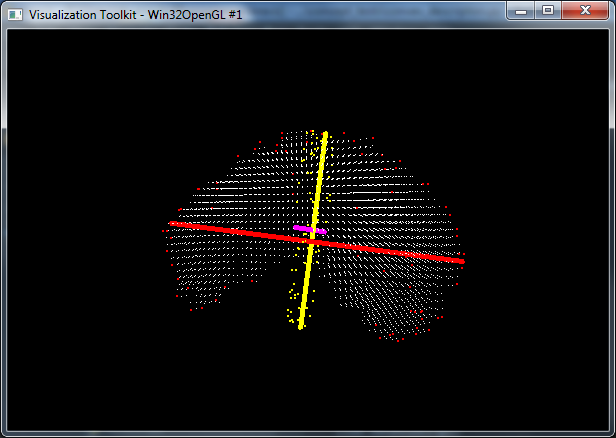
\includegraphics[width=0.9\textwidth]{figures/kmc400/desc_4}
	\caption{Illustration of the geometric descriptors calculated in python, white dots are the center of voxels that belong to a given structure, red points are those in the convex hull, the red line is the mayor axis of the structure, yellow points are the points in the structure projected to a plane perpendicular to the main axis, the yellow line is the mayor axis of this plane, finally the purple line is the axis perpendicular to the red and yellow axes.}
	\label{fig_jth_descs}
\end{figure}

DWI data was processed using Camino and the Free Surfer brain masks as references. Transformations between diffusion space and structural MRI space were calculated using \emph{FSL FLIRT}. From Camino we obtained FA, MD and color DTI maps, as well as full brain tractography. All of these were integrated into Braviz and made available for the experts. Additionally by using python scientific libraries and vtk we were able to combine Free Surfer data with tractography in order to isolate bundles going through particular structures. Mean FA, mean MD, mean length and number of tracks in the bundle were extracted for each bundle of interest.  While this could be achieved without Braviz, it was certainly easier using the infrastructure provided by the software. Additionally Braviz was used to let experts define spherical regions of interests and, based no them, define additional bundles of interest. The same scalar metrics mentioned before were extracted for these bundles. 

Additionally DWI data was processed using Free Surfer's Tracula. Output statistics were exported into the database and the probability maps of the bundles were integrated into Braviz for visualization. 

Functional MRI data was pre-processed in SPM.  After that a first level analysis was performed using specific contrasts for each paradigm, followed by a second level analysis using the main groups as regressor. The results from this analysis can be seen in \autocite{uriza_reporte_2015}. The Braviz \emph{fMRI Explore} tool was particularly useful in the first level stage as it displayed contrasts in a direct and clear way. Figure \ref{fig_spm_contrast_error} shows a problem with a contrast, because the left and right conditions are not of the same length. This problem was quickly identified and corrected.

\begin{figure}
	\centering
		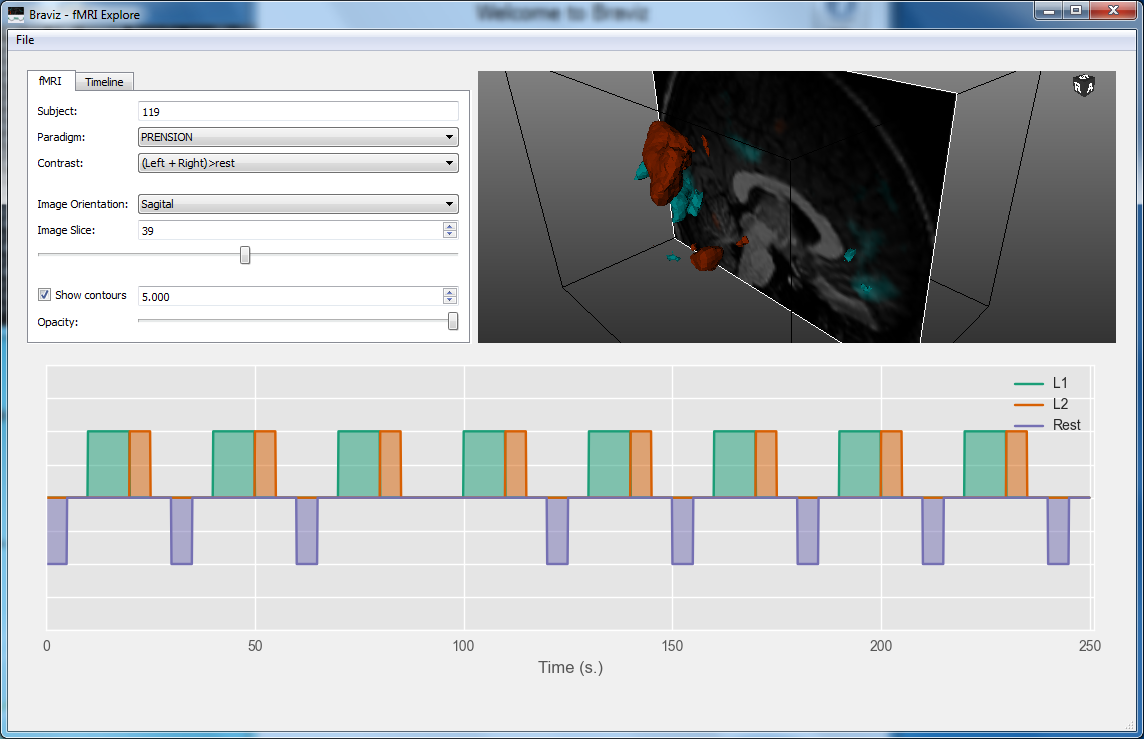
\includegraphics[width=0.9\textwidth]{figures/kmc400/erroro_fmri2}
	\caption{A problematic f-MRI contrast, L1 and L2 should have the same length.}
	\label{fig_spm_contrast_error}
\end{figure}
 

\subsection{Future Work}

The analysis of the data collected in this project is still far from finished. The crude analysis described above, which is simply regressing on each outcome variable against the exposition variable, is not enough to describe this data-set. Reality is much complex and several factors must be taken into account to perform a meaningful analysis. It requires defining the sample carefully and choosing a meaningful set of confounders. Also it is interesting to look at relationships that don't include the exposure variables, in order to get a better understanding of the factors that affect the development of preterm kids. 

For the moment only basic analysis have been done on spatial data. The information that can be extracted using scalars is limited, probably more interesting hypotheses can be discovered by making use of the totality of the data. However this will require the use of better tools and methodologies. Several second level analyzes will need to be performed using the SPM framework, as well as TBSS analyzes and shape analysis. This will have to be complemented with visual analysis of the data performed by domain experts. This will require new visualization options that can work at this scale. It would also be interesting to analyze the raw data captured during the TMS experiments (EMG signals) in order to find more complex relationships that the ones found using the derived scalars. 

Another challenge is looking at the behaviur of the cohort through time. This is analyzing the stability or variability of the different dimensions at the different epochs of in which data is available, and looking at the factors which determine this changes.

All data collected during this study will be made available on request to interested researchers from around the world. The objective is to improve the understanding of the different factors that affected the development of this cohort. At this point data must be used for hypotheses generation through exploratory analyzes. Confirming those hypotheses will likely require gathering additional data.

%Future
%Group analysis
%Mas analisis
%¿Se va a publicar la base de datos?


\section{Selected Braviz contributions}

%quality control
\subsubsection{Quality Control}

Gathering data and collecting it in a database in a project of this magnitude is large and complex task. Several steps are required and each of them several things can go wrong. Therefore guaranteeing quality of the data is not trivial. Data has to be continuously checked, validated and corrected as the project moves forward. This labor can benefit from automatic tools that check for values that are outside of range, are missing or which don't add up with other values. However large amounts of manual inspecting is also required. 

Anomalies in the data are much easier to detect when data is presented in graphical form then when presented in a table. A famous example of this is the Anscombe's Quartet \autocite{anscombe_graphs_1973}. The Braviz software can be used to visually explore data even as it is been acquired. Visualizations can be created and re visited again when more data is available. By looking at plots from the data strange values jump. This values can be instantaneously identified and verified from the raw data. Results from all analyzes are always accompanied by plots, which provides another sanity check. Any bizarre values will become evident and therefore the danger of believing results based on pathological data is reduced.

Verifying image data is also simple using tools from Braviz. The setup we used the most was several \emph{Subject Viewer} applications showing different critical slices of the image. An expert in radiology could then cycle through the subjects using the keyboard, and asses the quality. By using the platform it was possible to go over two hundred subjects in an hour. Images that appeared strange at first sight would be further evaluated by navigating in the 3d Viewer. Likewise quality of the registration between the different moralities could be checked by for example displaying the corpus callosum segmentation on top of an FA image. 

%fibers analysis
\subsubsection{Fiber Bundles Creation}

As the project advanced, questions related to different pathways in the brain started to emerge. In order to answer these questions it was necessary to isolate in the tractography the involved bundles. Some of these could be defined using structures segmented by freeSurfer, and therefore could be easily extracted for all subjects. However some of them required more precise location of waypoints. For this purpose the \emph{Roi Builder} application was created. With this application an expert could specify the precise location for a region of interest in a single subject taken any of the available images as context or cortical reconstructions. He could also receive instant feedback on the bundle of fibers that crossed the specific region. After positioning the spherical region on one subject, the application could approximate the equivalent location for the rest of the sample by using the available linear or non linear registration. These locations would afterwards need to be revised and adjusted by the expert, but the interface was built to make this process as efficient as possible.

The \emph{Logic Bundles} application provided even more freedom in defining custom fiber bundles. In this application the expert can use logical operations to define a bundle using several waypoints. These can be freeSurfer segmented structures or regions of interest created in other application. There can be mandatory waypoints, alternative waypoints and waypoints that must be avoided. 

Finally, after the bundles were defined, the system could be used to automatically extract scalar values from them. 


%sharing, presentations

\subsubsection{Data exploration}

One of the main purposes of Braviz was enabling researchers to quickly find potential relationships in the data that deserved a closer look. Displaying data visually lets the human visual system find odd aspects, which can lead the experts to think of new possibilities. 

Figure \ref{fig_anova_example} shows the plot of an ANOVA analysis between the volume of the left caudate nucleus. The plot shows that the most fragile subjects tend to have smaller caudate nuclei in both groups, however this relationship is not statisticially significant. Nevertheless it is worth taking a closer look and analyze if there is a biological justification for the relationship. If this is the case, maybe it is worth collecting more data in order to test this new hypothesis. Figure \ref{fig_caudate_parallel} shows another view of this relationship, this time showing left and right caudate nuclei. From the plot it can be seen that for most subjects both nuclei tend to have the same volume, and these are negatively related to the fragility index. It also calls our attention an outlier who has a strong asymmetry. Figure \ref{fig_asymetric_caudate_detail} shows this outlier on the \emph{Subject Overview} application; where it can be confirmed that the asymmetry is real. This can be seen directly on the image as well as on the notes written by the radiologist.


\begin{figure}
	\centering
		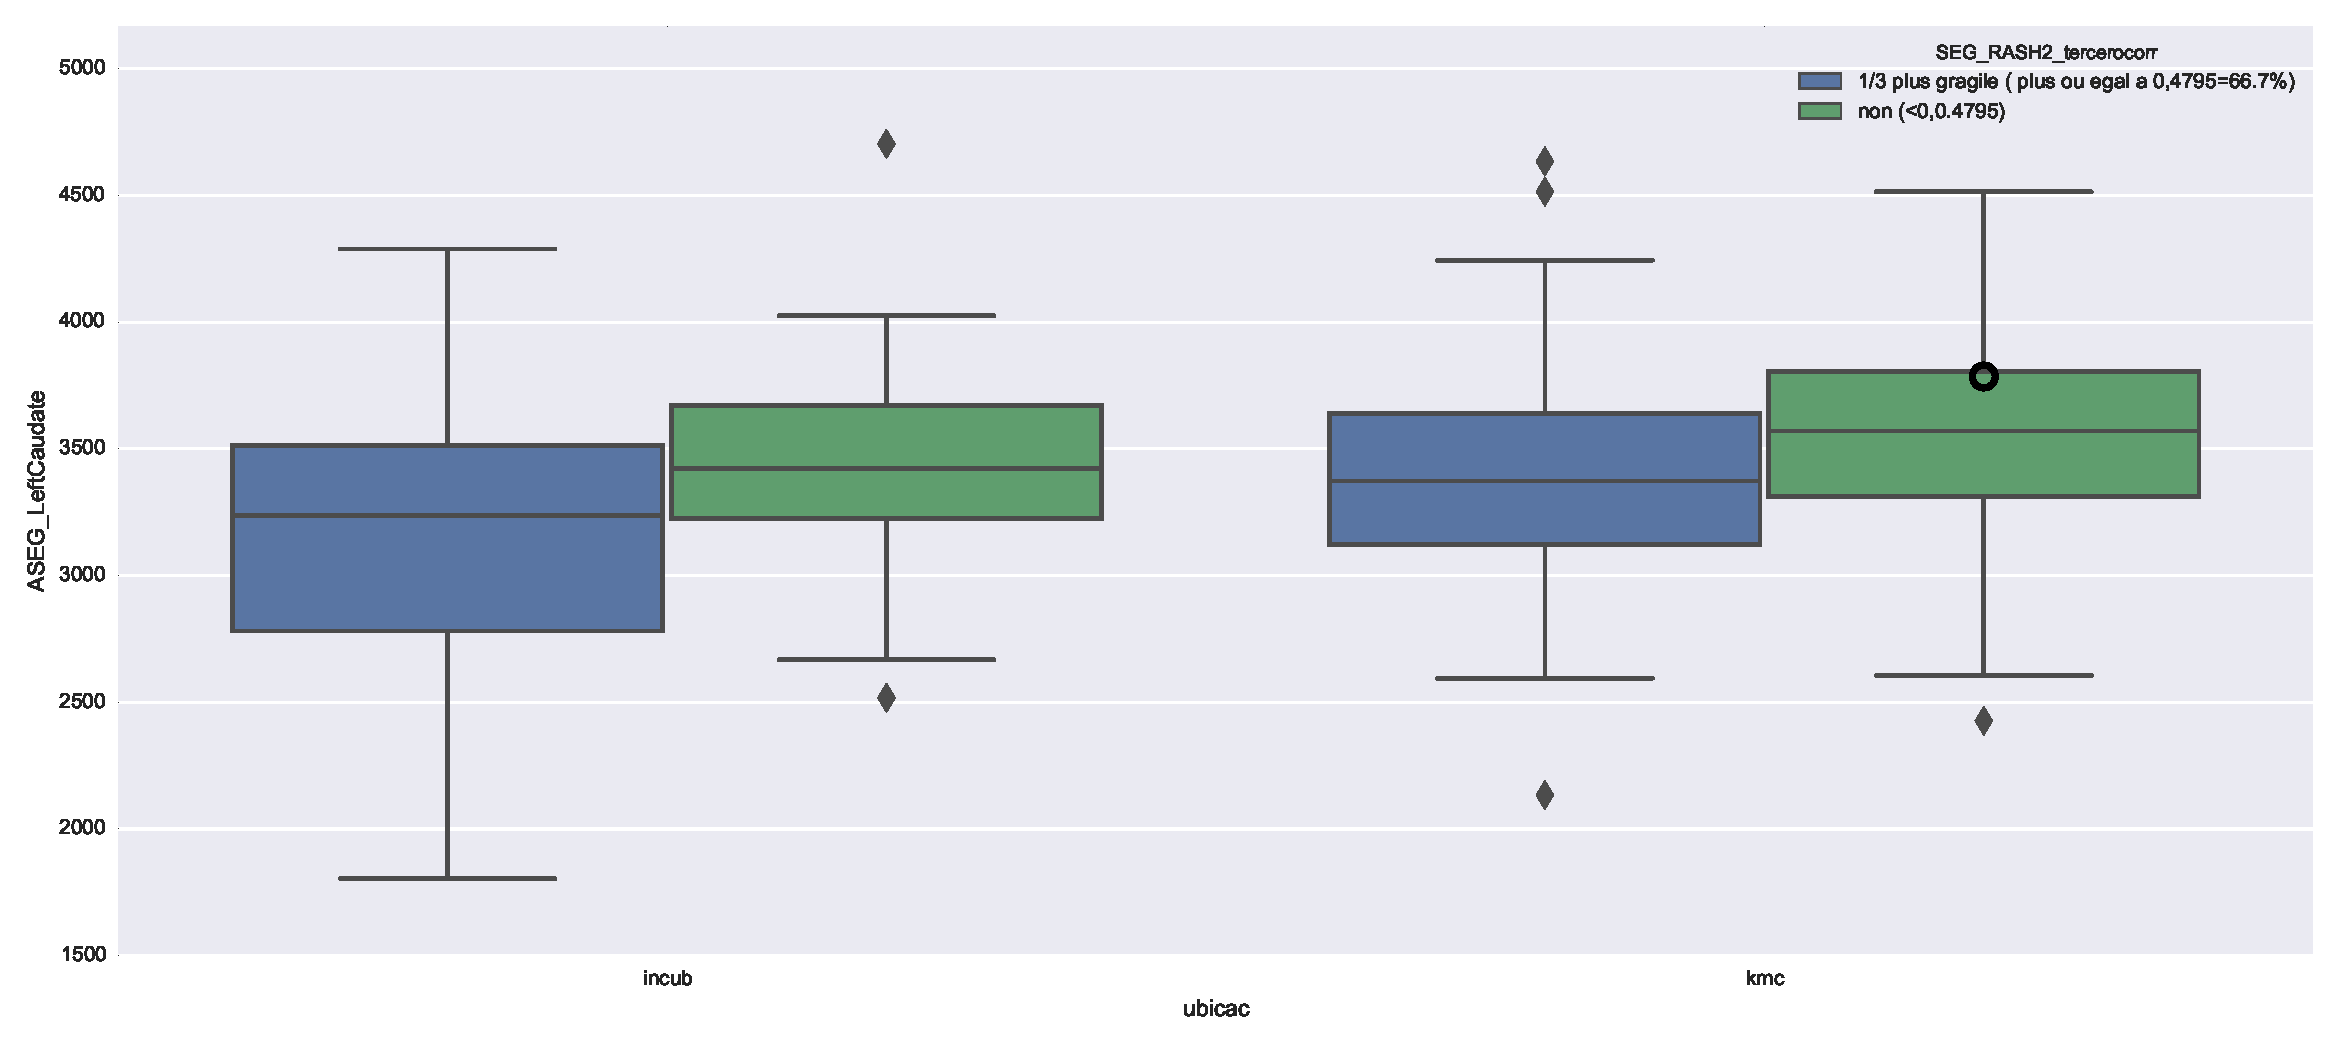
\includegraphics[width=\textwidth]{figures/kmc400/left_caudate_fragility_anova}
	\caption{An anova analysis of the volume of the left caudate nucleus against a fragility index and the treatment variable}
	\label{fig_anova_example}
\end{figure}


\begin{figure}
	\centering
		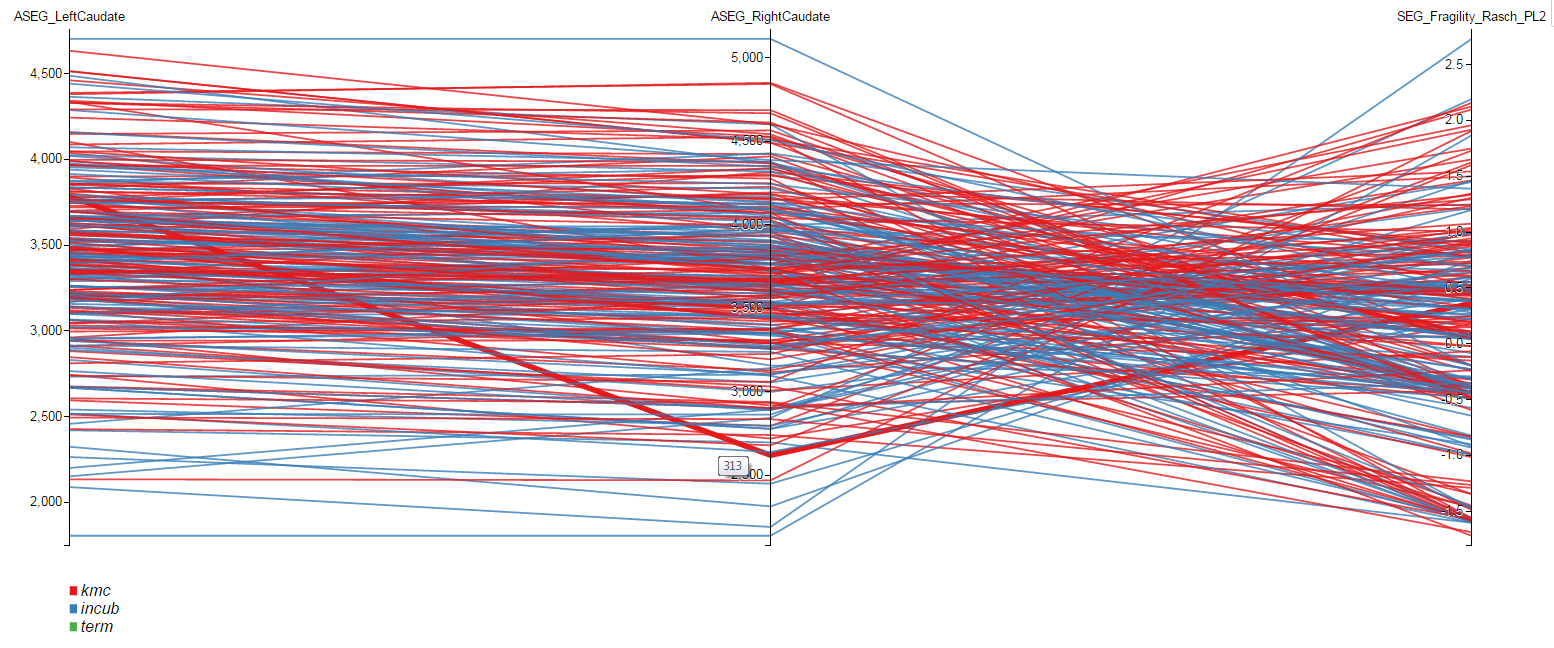
\includegraphics[width=\textwidth]{figures/kmc400/caudate_parallel}
	\caption{A parallel coordinates view of the left and right caudates in relationship with the fragility index. There is a clear negative correlation between the volumes of these structures and the fragility index, and a clear outlier.}
	\label{fig_caudate_parallel}
\end{figure}


\begin{figure}
	\centering
		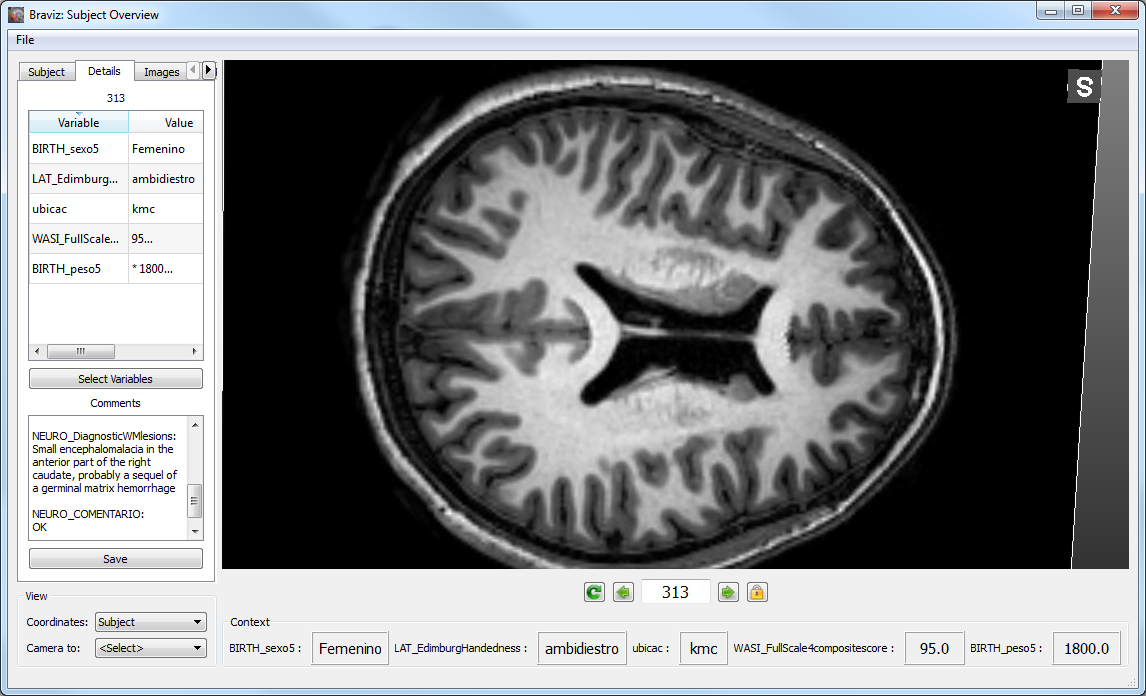
\includegraphics[width=\textwidth]{kmc400/caudate_detail}
	\caption{Detailed view of the outlier from figure \ref{fig_caudate_parallel}, it confirms that the strange behaviour exhibited is real and not a problem with the data.}
	\label{fig_asymetric_caudate_detail}
\end{figure}

% - Exploratory Analysis

% -- Use cases with Nathalie

% -- Examples of obvious and non obvious findings


%
%\begin{itemize}
%	\item Cognitive
%	\begin{itemize}
%		\item WASI II: Abbreviated intelligence test
%		\item TAP: Attention test
%		\item CVLT: Verbal learning test
%	\end{itemize}
%	\item Life Quality
%	\begin{itemize}
%		\item Kidscreen: Health related quality of life questionnaire.
%		\item Life habits questionaire: ???????
%		\item Pediatric Quality of Life Inventory : ??????????
%	\end{itemize}
%	\item Mental Health
%	\begin{itemize}
%		\item CES-D: Depression self report
%		\item Conners: ??????????????????????		
%	\end{itemize}
%	\item Behavior
%	\begin{itemize}
%		\item ABCL: Behavior checklist, completed by parents and best friend
%		\item ASR: Acute stress response
%		\item Rosemberg: Self-esteem questionnaire
%		\item Apego ?????????????
%	\end{itemize}
%	\item Neurosensorial 
%	\begin{itemize}
%		\item Optometry: Full sight evaluation
%		\item Audiometry: Full hearing evaluation
%		\item Edimburg laterality inventory: Dominant hand for multiple tasks
%		\item Nine Holes Peg Test: Manual dexterity
%		\item Beery Visuo-Motor Integration: Assesses integration between visual and motor abilities by copying images from a booklet.
%	\end{itemize}
%	\item Environment
%	\begin{itemize}
%		\item ?????????????????
%	\end{itemize}
%	\item Academic Performance
%	\begin{itemize}
%		\item ICFES: Results from the state high-school evaluation
%		\item School performance: Data of how the kids performed at school.
%		\item Current activity: Are the kids working or studying? If they work, what kind of work? what is the wage?
%	\end{itemize}
%	\item TMS % ¿Se aplicó a todos?
%	\begin{itemize}
%		\item Rest motor threshold
%		\item MEP (Motor Evoked Potential) Latency
%		\item Intra-cortical inhibition
%		\item Intra-cortical facilitation
%		\item Inter-hemispheric inhibition
%	\end{itemize}
%\end{itemize}